\chapter{Simulation}
\label{simulation}
A 6-DOF flight simulator was used to validated the drag prediction method before hardware was purchased. The main utility of the simulator was to provide simulated flight test data with signals that contained no noise. The actual sensors during a flight test will be noisy signals, and Guassian white noise can be added to the clean signals to check the method's sensitivity to sensor noise.

\section{Simulation Environment}
The flight simulator used was a model of the de Haviland Beaver that comes as a demo in the Aerospace Toolbox of Simulink. The Simulink model was modified to output required signals to the workspace, which essentially created a sensor with zero noise. The mass, moments of inertia, and reference lengths were then scaled to those of a Zagi R/C aircraft found in \cite{stevens2003aircraft}. The original Simulink model was already connected to a Flight Gear visualization engine, but the model was altered such that the indicators would function properly.

\section{Simulation Inputs}
The engine forces and moments were set to zero in the simulator, to match the assumption of a folding propeller.
The force calculations built into the Beaver Simulink model were replaced with a parabolic drag polar of the form
\begin{align}
C_D &= C_{D_0} + K*(C_L(\alpha)-C_{L_{min}})
\end{align}

The lift coefficient $C_L(\alpha)$ was nonlinear aerodynamic data from a NACA 0012 taken from \cite{osborne2007transitions}. While this approximation to a nonlinear drag polar does not capture the drag rise due to stall, it does represent the limited lifting capability of a real wing, making it more realistic than assuming the wing does not stall.
\section{Simulation Results}
The most first result of the simulation testing was a verification of the correct equations of motion. The simulation was initialized with various initial states to ensure there was no dependence on initial conditions. The vehicle was then flown by an R/C aircraft pilot using a joystick attached the to simulation. It was noted early in the simulation testing that flying a sweep of speeds was beneficial, as a wider range of the drag polar was flown. This result was included in much of the flight test planning.
One of the main goals of the simulation was to verify the data analysis routines developed in Matlab did in fact match inputs to outputs. To do this, the simulation was flown and, when finished, no noise was added to the data. The results are shown in Figure \ref{dragPolarNoNoise}.

\begin{figure}[h!]
  \caption{Equations of Motion Verification (No Noise)} \label{dragPolarNoNoise}
  \centering
    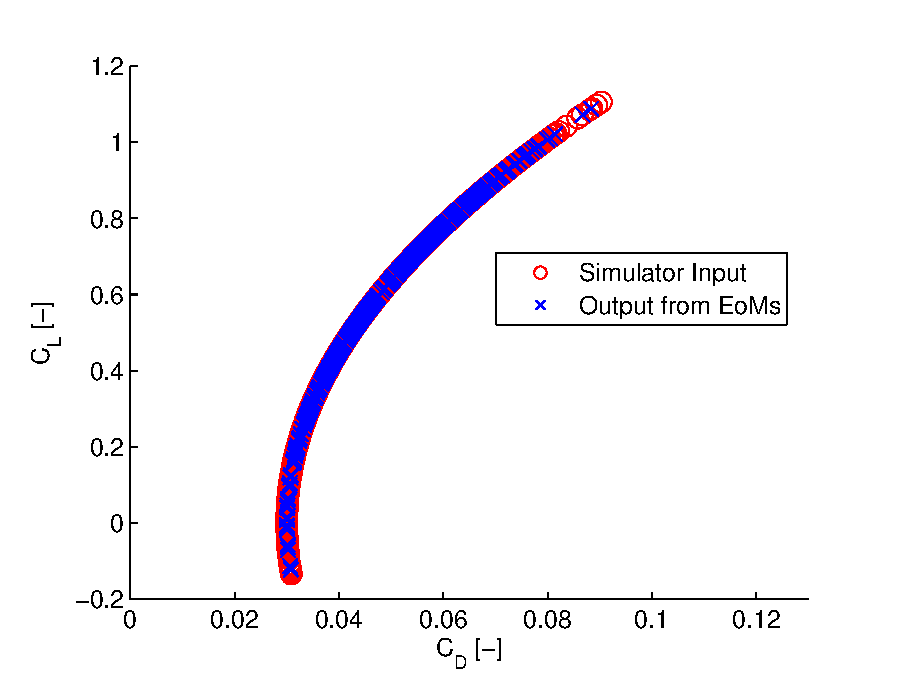
\includegraphics[width=0.5\textwidth]{figures/dragPolarNoNoise.eps}
\end{figure}

Figure \ref{dragPolarNoNoise} shows that the equations of motion used in the data analysis functions properly calculate the coefficients being passed into the system. With this result, noise was added to the system to see how sensitive coefficient estimation was to noise in each sensor. This process was a balancing act between available sensor accuracy and accuracy of the final solution. The final result guided sensor selection to those discussed in Section \ref{hardware}. To check if the final sensors chosen were acceptable, Gaussian noise was added to each state, with a mean of $0$ and a standard deviation equal to the root-mean-squared error listed in the manufacturer's data sheet for each sensor.
\begin{figure}[H]
  \caption{Drag Polar Prediction of Simulated Test Flight} \label{dragPolarNoise}
  \centering
    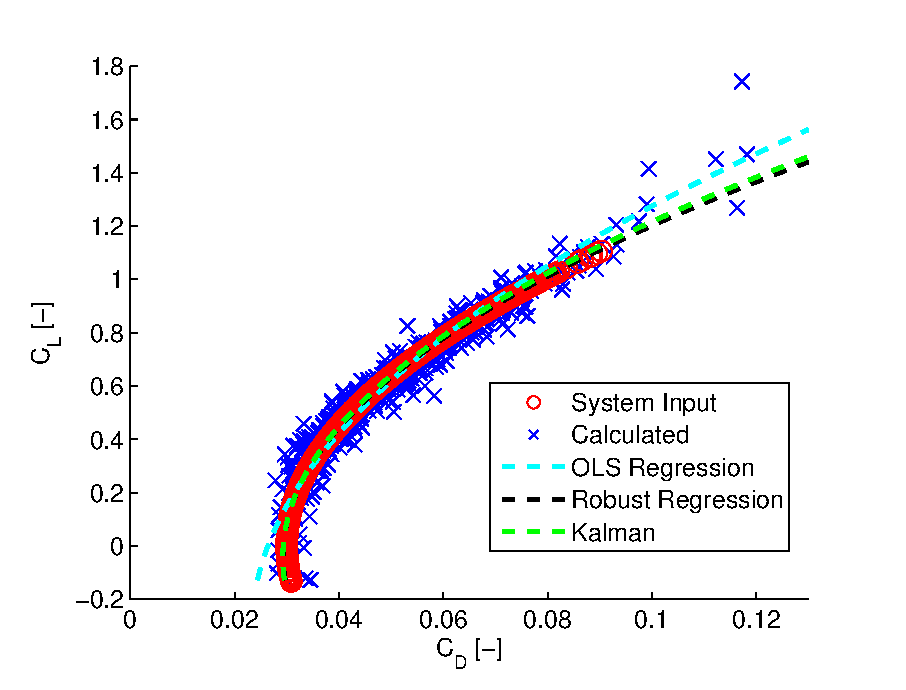
\includegraphics[width=0.5\textwidth]{figures/simDragPolarNoise.eps}
\end{figure}

For the particular simulated test flight shown in Figure \ref{dragPolarNoise}, the estimated drag polar coefficients had error coefficients outlined in Table \ref{simCoeffErrorTable}.

\begin{table}[ht]
\caption{Nonlinear Model Results} % title of Table
\centering % used for centering table
\begin{tabular}{c c c c} % centered columns (4 columns)
\hline\hline %inserts double horizontal lines
 & $C_{D_0}$ & $K_1$ & $K_2$ \\ [0.5ex] % inserts table 
%heading
\hline % inserts single horizontal line
System Inputs & 0.0493 & 0 & 0.03 \\ % inserting body of the table
OLS Estimate & 0.0516 & -0.0056 & 0.0317 \\
Robust LS Estimate & 0.0500 & -0.0035 & 0.0313 \\ [1ex] % [1ex] adds vertical space
\hline %inserts single line
\end{tabular}
\label{table:nonlin} % is used to refer this table in the text
\end{table}

The results of this simulated flight test showed that the measurement system outlined in Section \ref{hardware} predicted the simulated drag polar with a reasonable error.